\documentclass[12pt]{article}
\usepackage[utf8]{inputenc}
\usepackage{geometry}
\geometry{a4paper, margin=1in}
\usepackage{graphicx}
\usepackage{hyperref}
\usepackage{amsmath}
\usepackage{pgfplots}
\pgfplotsset{compat=1.18}

\title{Projeto Abrangente 0001}
\author{Gerente de Projeto: John Doe}
\date{24 de setembro de 2024}

\begin{document}

\maketitle

\tableofcontents
\newpage

\section{Introdução}
Este memorando de projeto abrangente fornece uma atualização detalhada sobre o projeto ABC, descrevendo o progresso, os principais riscos, as estratégias de mitigação e os próximos marcos. O memorando está estruturado para oferecer insights detalhados sobre cada fase do projeto e destacar áreas cruciais de foco para os próximos meses.

O objetivo do projeto é aumentar o desempenho do sistema em 30\%, tornando-o mais eficiente e escalável para requisitos futuros. Desde a última atualização em agosto, fizemos progressos significativos, mas ainda há desafios, particularmente na integração de APIs e otimização do banco de dados.

\section{Visão Geral do Projeto}
O projeto ABC está dividido em três fases:
\begin{itemize}
    \item \textbf{Fase 1: Levantamento de Requisitos} (Concluído)
    \item \textbf{Fase 2: Desenvolvimento} (Em andamento)
    \item \textbf{Fase 3: Testes e Implementação} (Programado)
\end{itemize}

\subsection{Fase 1: Levantamento de Requisitos}
A Fase 1 foi concluída em 15 de agosto de 2024. Durante esta fase, colaboramos com as principais partes interessadas para reunir requisitos abrangentes. Isso garantiu o alinhamento entre a equipe de desenvolvimento e os objetivos de negócios.

O processo de levantamento de requisitos revelou várias áreas de potencial melhoria, incluindo melhorar a segurança do sistema, escalar a infraestrutura para suportar usuários adicionais e integrar APIs de terceiros para aumentar a funcionalidade.

\subsection{Fase 2: Desenvolvimento}
A Fase 2, que começou em meados de agosto, foi dividida em duas principais frentes de trabalho: desenvolvimento do frontend e integração do backend.

\paragraph{Desenvolvimento do Frontend} A interface de usuário foi redesenhada para melhorar a experiência do usuário. O feedback da equipe de design sugere que a nova interface reduz a fricção do usuário, especialmente em ambientes de alto tráfego.

\paragraph{Integração do Backend} O sistema backend está passando por atualizações significativas, incluindo:
\begin{itemize}
    \item Implementação de uma arquitetura de microsserviços.
    \item Melhoria na gestão de banco de dados.
    \item Integração de APIs.
\end{itemize}

Atualmente, enfrentamos atrasos na integração das APIs do backend, o que impactou o cronograma do projeto. No entanto, estamos adicionando recursos adicionais para garantir que este atraso não se prolongue para a próxima fase.

\section{Status Atual}
Até 24 de setembro de 2024, fizemos progressos significativos tanto no desenvolvimento do frontend quanto na integração do backend.

\subsection{Métricas de Progresso}
A tabela a seguir fornece uma visão geral do progresso do projeto, descrevendo o percentual concluído para os principais componentes da Fase 2.

\begin{table}[h!]
\centering
\begin{tabular}{|c|c|c|}
\hline
\textbf{Componente} & \textbf{Data de Conclusão Prevista} & \textbf{Progresso (\%)} \\
\hline
Desenvolvimento do Frontend & 5 de outubro de 2024 & 80\% \\
Desenvolvimento do Backend & 20 de outubro de 2024 & 60\% \\
Integração de APIs & 1 de outubro de 2024 & 50\% \\
Otimização de Banco de Dados & 10 de outubro de 2024 & 70\% \\
\hline
\end{tabular}
\caption{Resumo de Progresso dos Componentes Principais}
\end{table}

\subsection{Gráfico de Burndown de Desenvolvimento}
Abaixo está um gráfico de burndown que mostra o progresso da equipe nas últimas seis semanas. Ele rastreia o trabalho restante em relação ao trabalho planejado para a Fase 2.

\begin{center}
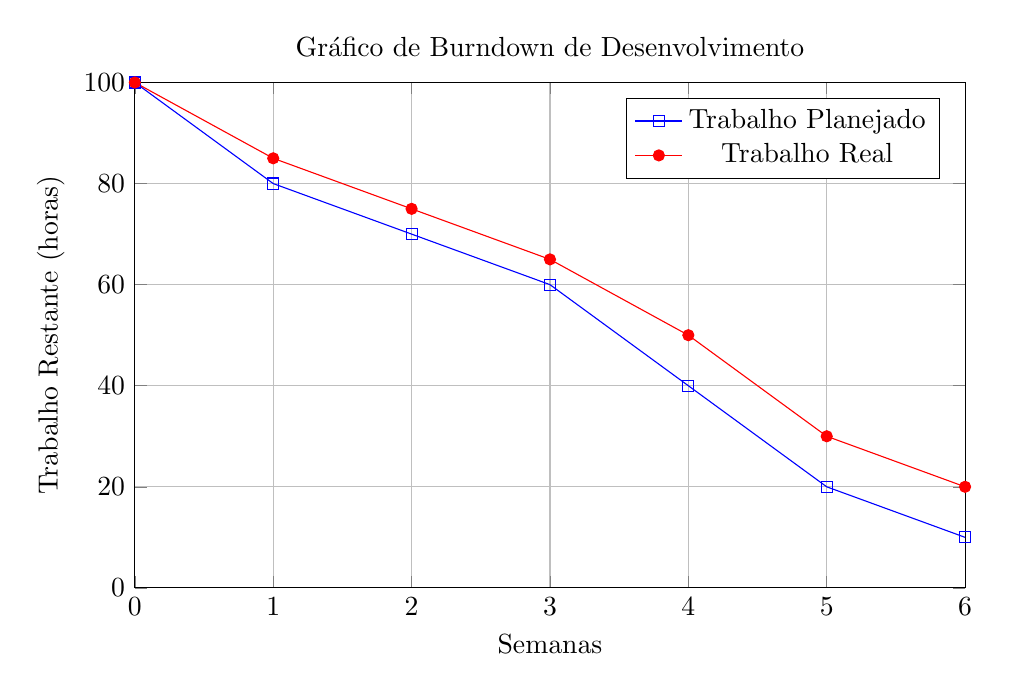
\begin{tikzpicture}
\begin{axis}[
    title={Gráfico de Burndown de Desenvolvimento},
    xlabel={Semanas},
    ylabel={Trabalho Restante (horas)},
    xmin=0, xmax=6,
    ymin=0, ymax=100,
    xtick={0,1,2,3,4,5,6},
    ytick={0,20,40,60,80,100},
    legend pos=north east,
    grid=major,
    width=\linewidth,
    height=8cm
]
\addplot[color=blue,mark=square] coordinates {
    (0, 100) (1, 80) (2, 70) (3, 60) (4, 40) (5, 20) (6, 10)
};
\addplot[color=red,mark=*] coordinates {
    (0, 100) (1, 85) (2, 75) (3, 65) (4, 50) (5, 30) (6, 20)
};
\legend{Trabalho Planejado, Trabalho Real}
\end{axis}
\end{tikzpicture}
\end{center}

\newpage
\section{Principais Riscos e Estratégias de Mitigação}
Vários riscos foram identificados, com as correspondentes estratégias de mitigação descritas a seguir:

\subsection{Risco 1: Atrasos na Integração de APIs}
\textbf{Descrição:} Os atrasos na integração de APIs de terceiros criaram um gargalo no desenvolvimento do backend. Isso pode adiar a conclusão do backend em duas semanas.

\textbf{Estratégia de Mitigação:} Um desenvolvedor adicional foi designado para a equipe de integração de APIs para acelerar o processo. Também estamos em discussões com o fornecedor externo para agilizar as mudanças necessárias.

\subsection{Risco 2: Problemas de Escalabilidade do Banco de Dados}
\textbf{Descrição:} Testes iniciais revelaram possíveis problemas de escalabilidade do banco de dados. Isso pode causar gargalos de desempenho quando o sistema estiver sob carga pesada.

\textbf{Estratégia de Mitigação:} A equipe de arquitetura está revisando o design do banco de dados. Planejamos implementar uma solução de escalabilidade horizontal que distribuirá a carga entre várias instâncias de banco de dados.

\section{Próximos Marcos}
Os próximos passos do projeto incluem os seguintes marcos chave:

\begin{itemize}
    \item \textbf{1 de outubro de 2024:} Completar a integração de APIs.
    \item \textbf{10 de outubro de 2024:} Iniciar testes abrangentes do sistema, incluindo testes de desempenho e segurança.
    \item \textbf{20 de outubro de 2024:} Concluir o desenvolvimento do backend, incluindo a otimização do banco de dados.
    \item \textbf{5 de novembro de 2024:} Iniciar a implementação gradual em ambientes de staging.
    \item \textbf{15 de novembro de 2024:} Implementação final em produção.
\end{itemize}

\section{Conclusão}
O projeto ABC está progredindo bem, embora ainda restem alguns riscos, particularmente na integração de APIs e na escalabilidade do banco de dados. Com os recursos adicionais alocados ao projeto e a estreita colaboração com fornecedores externos, esperamos cumprir os prazos revisados. Uma atualização detalhada será fornecida no próximo memorando do projeto, programado para 24 de outubro de 2024.

\end{document}
